

\section{Conectores Molex}
\label{conectores_01}


\begin{table}[ht!]

	\begin{tabular}{r l|l p{12cm} }
		
		\textcolor{gray}{Especificação} &&& 	{Conectores Molex}\\
		\textcolor{gray}{Data} &&& 				{14/10/2014}\\
        \textcolor{gray}{Beneficiado} &&&		{Dova Equipamentos Eletricos LTDA}
        \\
        \textcolor{gray}{CNPJ} &&& 				{33.462.359/0001-30} \\
        \textcolor{gray}{Número Nota} &&& 		{000.004.382} \\
		\textcolor{gray}{Quantidade} &&& 		{-} \\
		\textcolor{gray}{Valor} &&& 			{R\$165,00} \\
		\textcolor{gray}{Data Sheet} &&& 		{-} \\

		\textcolor{gray}{Função no projeto} &&& {Os conectores molex são necessários
		para a integração dos circuitos e sensores dentro da eletrônica embarcada. Os
		cabinhos de silicone 0.75mm2 realizam as conexões internamente.}
		\\
		\textcolor{gray}{Razão da Escolha} &&& {A empresa Dova fornece conectores
		molex para o laboratório em pronta entrega e de baixo custo.}

	\end{tabular}
\end{table}

\newpage
\subsection{Foto do Material}
\begin{figure}[H]
 \centering
 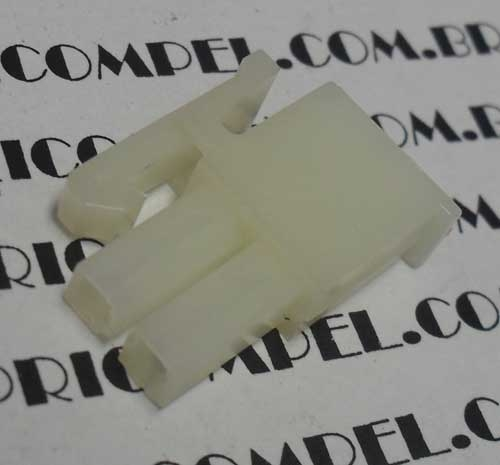
\includegraphics[width=1\columnwidth]{Conectores_01/foto.jpg}
 \caption{Conector Molex 2 vias}
\end{figure}

\subsection{Nota Fiscal}
\begin{figure}[H]
 \centering
 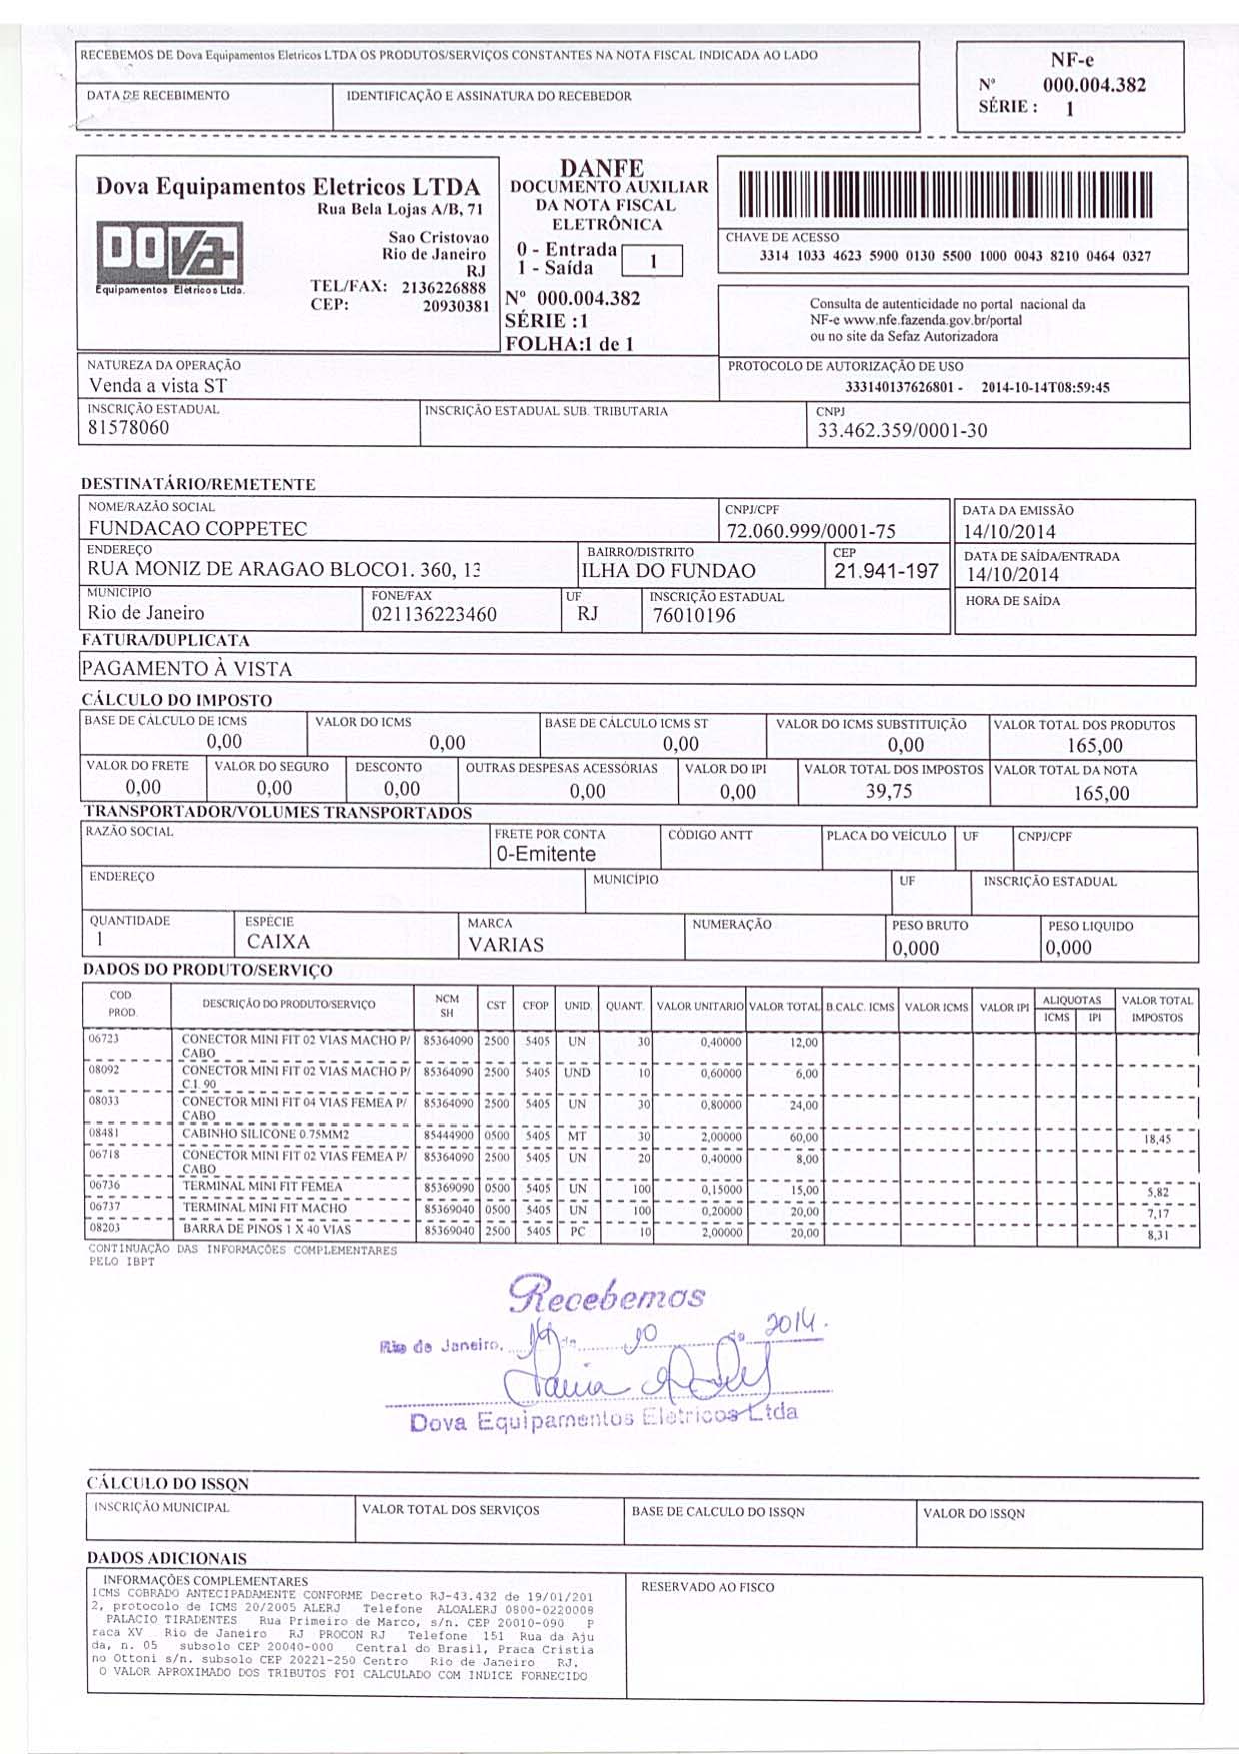
\includegraphics[width=0.9\columnwidth]{Conectores_01/nota_dova.pdf}
 \caption{Conectores Molex - Dova}
 \end{figure}